\documentclass[a4paper,twoside,12pt,DIV=13,BCOR=5mm,numbers=noenddot,cleardoublepage=empty]{scrbook}
%======= Einbinden der benötigten Packete (= Zusatzfunktionen)
\usepackage[T1]{fontenc}                % für Fonts in westeuropäischer Codierung
\usepackage{lmodern}										% Latin Modern Paket verändert die verwendete Schriftart. Bessere Darstellung für pdf
\usepackage{textcomp}										% Provides extra symbols, e.g. arrows like \textrightarrow, various currencies (\texteuro,..
\usepackage[latin1]{inputenc}    				% german special characters
\usepackage[english,ngerman]{babel}     % hyphenation   usepackage[english,ngerman]{babel} f. deutsch
\usepackage{pdfpages}										% Einbinden von pdf-Files
\usepackage{pifont,textcomp,mathcomp}   % dingbad psfonts and text-compilant fonts (euro, TM, ...)
\usepackage{amsmath,amsopn,amsthm}      % AMS mathematics
\usepackage{amssymb}                    % zusätzliche Symbole 
\usepackage{xspace}											% avoids eaten spaces

%======= Eine Umgebung für Bilder und Tabellen			  	
%\usepackage[textfont={Small},labelfont={bf},margin=1cm,format=plain,font=singlespacing]{caption}   % hanging caption text [hang]
\usepackage[textfont={small},labelfont={bf},margin=1cm,format=plain,font=singlespacing]{caption}   % hanging caption text [hang]
\captionsetup*[figure]{name=Abb.}			 % Abbildungsunterschrift beginnt mit Abb.
\captionsetup*[table]{name=Tab.}


%======= Farben für Überschriften
\usepackage{color}
\definecolor{TUBlau}{rgb}{0,0.4,0.6}   % TU-blau RGB 0 102 153
\addtokomafont{sectioning}{\sffamily\bfseries\selectfont\color{TUBlau}}
\setkomafont{chapter}{\normalfont\huge\sffamily\bfseries\color{TUBlau}}
\addtokomafont{section}{\Large}
\addtokomafont{subsection}{\normalfont\Large\sffamily\bfseries\color{TUBlau}}
\addtokomafont{subsubsection}{\normalfont\large\sffamily\bfseries\color{TUBlau}}
\addtokomafont{paragraph}{\normalfont\large\sffamily\bfseries\color{TUBlau}}


%======= Kopf-/Fußzeilen
\pagestyle{plain} % nur Fußzeile



%======= Eine kompakte Umgebung für die Bilder
\newcommand{\bild}[4]{{
\begin{figure}[#2]
\begin{center}
\includegraphics[scale=#3]{pictures/#1}
\caption{#4}\label{fig:#1}
\end{center}
\end{figure}
}}


%======= Definitionen eigener Befehle
\newcommand{\degC}{\ensuremath{^{\circ}}C}        % Grad Celsius
\newcommand{\Gu}{\glqq{}}                         % Gänsefüßchen unten
\newcommand{\Go}{\grqq{}\xspace}    												% Gänsefüßchen oben











 
\usepackage{graPhicx}
\usepackage{esvect}
\usepackage{bm}
\usepackage{mathtools}
\begin{document}
    \renewcommand{\baselinestretch}{1.25}
    \newcommand{\StudentA}{Philipp Hanser}
    \newcommand{\MatrNrA}{11775264}
    \newcommand{\StudentB}{Florian Strebl}
    \newcommand{\MatrNrB}{11712190}
    \newcommand{\StudentC}{Alexander Seiler}
    \newcommand{\MatrNrC}{11771276}

    \newcommand{\LUDatum}{06.06.2019}
    \newcommand{\LUGruppe}{Gr. 15}
    \newcommand{\LUBetreuer}{Geiginger, Lisa-Marie}  

    \large
    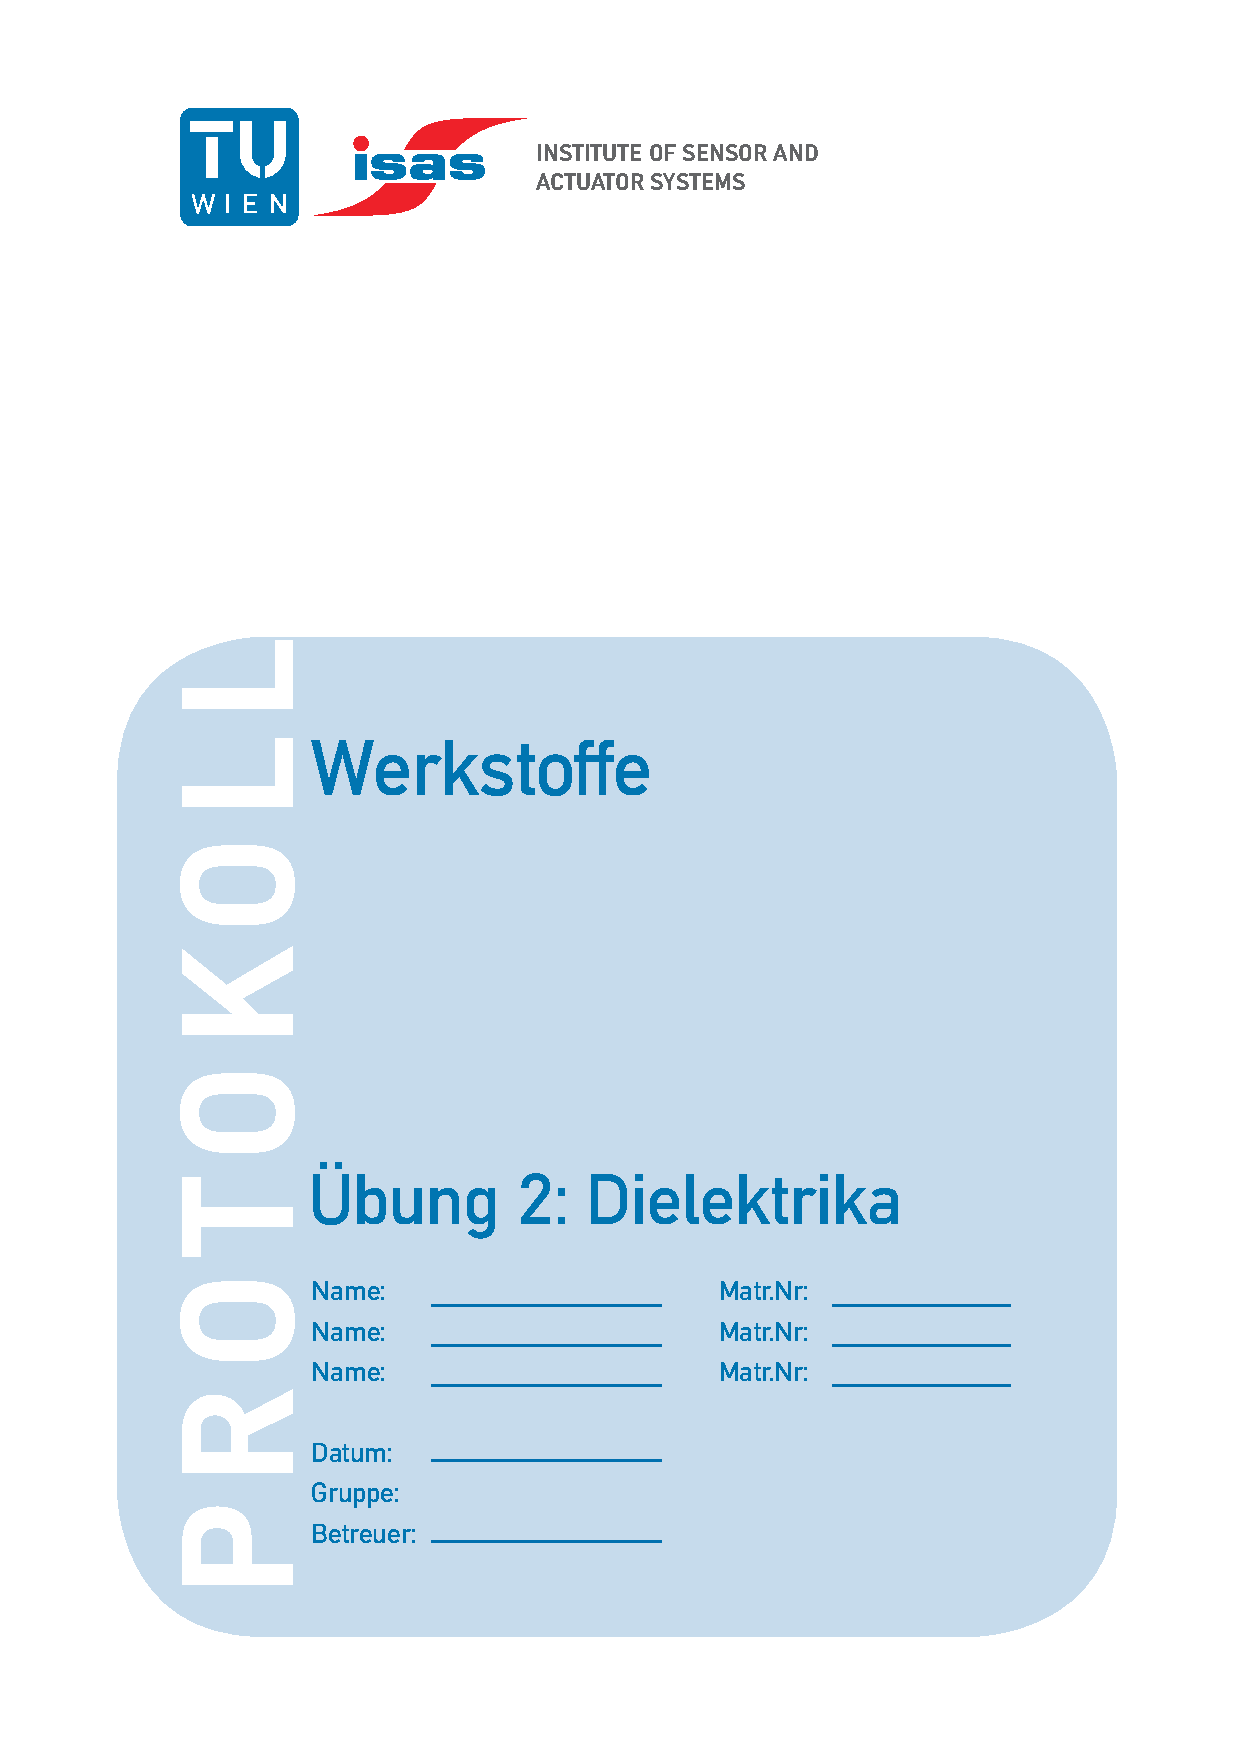
\includepdf[fitpaper=true,
                            picturecommand*={\unitlength1cm 
                            \put(7.3,7.7){\StudentA} \put(14.1,7.7){\MatrNrA}
                \put(7.3,7.0){\StudentB} \put(14.1,7.0){\MatrNrB}
                \put(7.3,6.3){\StudentC} \put(14.1,6.3){\MatrNrC}
                            \put(7.3,5.1){\LUDatum} 
                \put(7.3,4.4){\LUGruppe} 
                \put(7.3,3.7){\LUBetreuer} 
    }]
    {pictures/DeckblattLUDie}


    \setcounter{tocdepth}{3}

    \setcounter{page}{0}
    \renewcommand{\thepage}{\roman{page}}
    \tableofcontents \cleardoublepage

    \setcounter{page}{1}
    \renewcommand{\thepage}{\arabic{page}}
    \setcounter{chapter}{0}

    \chapter{Durchgangs- und Oberfl\"achenwiderstand}

    \chapter{Dieelektrizit\"atszahl}

    \chapter{Durchschlagsfestigkeit}
\end{document}